\documentclass[12pt]{article}
\usepackage[top=1in,bottom=1in,left=1in,right=1in]{geometry}
\usepackage{alltt}
\usepackage{array}	
\usepackage{graphicx}
\usepackage{tabularx}
\usepackage{verbatim}
\usepackage{setspace}
\usepackage{listings}
\usepackage{amssymb,amsmath, amsthm}
\usepackage{hyperref}
\usepackage{oz}
\usepackage[cc]{titlepic}
\usepackage{fancyvrb}


\title{\textbf{Concordia University
Department of Computer Science and Software
Engineering} \\ \ \\SOEN 331 Section S: Formal Methods\\for Software Engineering\\
 \\ 
Assignment 4}
\author{Mohammad Ali Zahir - 40077619 & Marwa Khalid - 40155098}
\date{November 23, 2022 \\ & \ \\ Date of Submission: December 2, 2022}
\begin{spacing}{1.5}
\begin{document}
\maketitle

\newpage
\tableofcontents
\newpage

\section{Our assignment}
\begin{enumerate}
\item (10 pts) Find a logically equivalent formula for $\phi \ W \ \psi$ and provide a short reasoning
to support your answer. Represent this equivalence between the two expressions with
the appropriate logical connective, and support your reasoning.\\\
\\
\noindent \underline{Solution}:\\ The logically equivalent formula for this would be:\\
\( (\phi \ \textbf{W} \ \psi) \equiv \ $(\phi \ \textbf{U} \ \psi$)\ \vee \ $\square(\psi)$ \\
\noindent These are equivalent, because the principle of the strong until operator \textbf{U}. Since the $\psi$ is never guaranteed to be true, we would need to add an extra or statement because if the statement $\psi$ becomes true it would mean that $\phi$ can't be true. This means that $\phi$ would be true until a certain condition ($\psi$ is true) is met. \\

\item (10 pts) Find a logically equivalent formula for $\phi \ U \ \psi$ , and provide a short reasoning
to support your answer. Represent this equivalence between the two expressions with the appropriate logical connective, and support your reasoning.\\\
\\
\noindent \underline{Solution}:\\ The logically equivalent formula for this would be: \\
$(\phi \ \textbf{U} \ \psi$) \equiv \  $(\phi \ \textbf{W} \ \psi) \ \wedge \ $\bigcirc \lozenge(\psi)$ \\
\noindent These are equivalent, because the principle of the strong until operator U. We know that this $\psi$ will eventually become true. We then now that we can use the weak until clause with an eventually operator, because the only way that $\phi$ is not true is when the $\psi$ is not true. We add the and operator, because we want to insure that the next one we actually get $\psi$ as being true, because this may never happen. \\

\item (10 pts) Find a logically equivalent formula for $\phi \ R \ \psi$ in terms of W , and provide a short reasoning
to support your answer. Represent this equivalence between the two expressions with the appropriate logical connective, and support your reasoning.\\\
\\
\noindent \underline{Solution}:\\ The logically equivalent formula for this would be: \\
$(\phi \ \textbf{R} \ \psi$) \equiv \ $(\phi \ \textbf{W} \ \psi) \ \wedge \ $\lozenge(\psi)$ \\
\noindent These are equivalent as the weak until will make the operation hold until something is triggered. We need the second part of the equation to guarantee that $\psi$ will eventually has to be true, because if it is not then, this will never hold. Hence the and statement. \\
\\
\noindent This paragraph refers to Questions 4 - 5: Consider a railroad with a single rail and a
road level-crossing. We introduce the following propositions that represent events:
\begin{itemize}
\item[] a : A train is approaching.
\item[] b : The barrier is down
\item[] c : A train is crossing
\item[] l: A light is blinking
\end{itemize}
\item (15 pts) Express each of the following requirements formally. For each one, proceed to
find a logically equivalent formula that captures the safety property of the system (i.e.
in terms of “something bad never happens”):
\begin{itemize}
\item[(a)] (5 pts) When a train is crossing, the barrier must be down. \\
\noindent \underline{Solution}:\\ 
\square $(c \rightarrow \square b)$
\item[(b)] (5 pts) If a train is approaching or crossing, then the light must be blinking.
\noindent \underline{Solution}:\\
\square $(a \vee c \rightarrow \square l)$
\item[(c)] (5 pts) If the barrier is up and the light is off, then no train is coming or crossing.
\noindent \underline{Solution}:\\
\square $(\lnot(b \wedge l) \rightarrow \lnot \square(a \vee c)) $
\end{itemize}
\item (10 pts) Express each of the following requirements formally in terms of the liveness
property (i.e. in terms of “something good eventually happens”):
\begin{itemize}
\item[(a)] (5 pts) When a train is approaching, it will eventually cross.. \\
\noindent \underline{Solution}:\\
\square $(a \rightarrow \lozenge c) $
\item[(b)] (5 pts) When a train is approaching and no train is crossing, then the barrier will
eventually go down before the train crosses. \\
\noindent \underline{Solution}:\\
\square $((a \wedge \lnot c) \rightarrow \lozenge(\lnot b \ \textbf{U} \ c)) $
\end{itemize}
\item (45 pts) The behavior of a program is expressed by the following temporal formula:\\

\begin{figure}[h!]
\centering
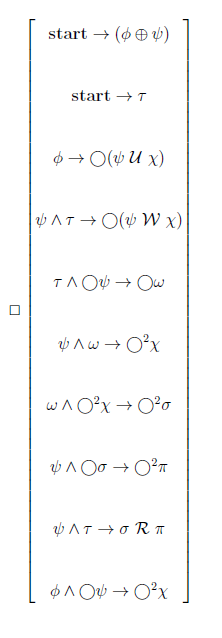
\includegraphics[width=0.9\textwidth, height = 15cm, keepaspectratio]{images/Q6.png}
\end{figure}
\begin{itemize}
\item[(a)](20 pts) Visualize all models of behavior. \\
\noindent \underline{Solution}:\\
\begin{figure}[h!]
\centering
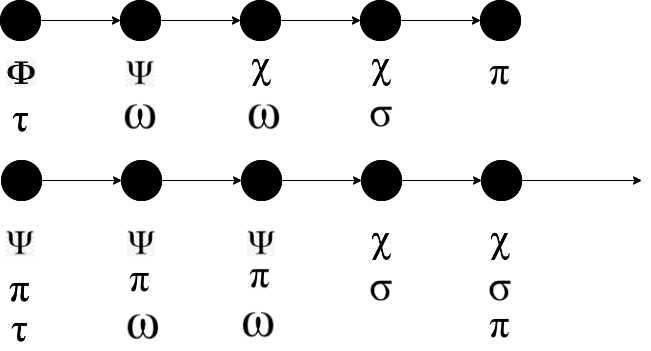
\includegraphics[width=0.9\textwidth, height = 15cm, keepaspectratio]{images/SOEN331_A4_Q6a.png}
\end{figure}
\begin{itemize}
\item[(b)](10 pts) Is the set of requirements satisfiable in all models of behavior? Explain
why or why not. \\
\noindent \underline{Solution}:\\ This set of requirements is not satistfiable in all behaviors. The first timeline, the top one terminates fine, hence it has no problems. The second one however has the operation $ \textbf{R} $ which means strong release. The specific condition that is using the strong release, would be the:
$\psi \wedge \tau \rightarrow \sigma \ \textbf{R} \ \pi $ \\
Hence at i =3, is when our strong release should have ended, but at i =4, we see an extra $ \pi $ which is not supposed to be there. \textbf{Hence this is not valid for all requirements}.  \\

\item[(c)] (10 pts) In the case where the set of requirements is not satisfiable, what modification(
s) to the requirements would you make (you may temporarily assume the
role of a stakeholder) in order to achieve satisfiability. \\
\noindent \underline{Solution}:\\
As the stakeholder, we are allowed to do change the program requirements how we want them to be. Hence the best way to acheive satisfiability would be the remove the condition that cause the problem in the second timeline which would be: \
$\psi \wedge \bigcirc \sigma \rightarrow \bigcirc^2 \pi $ \\
Hence after we remove that condition, our new timelines look like: \\
\begin{figure}[h!]
\centering
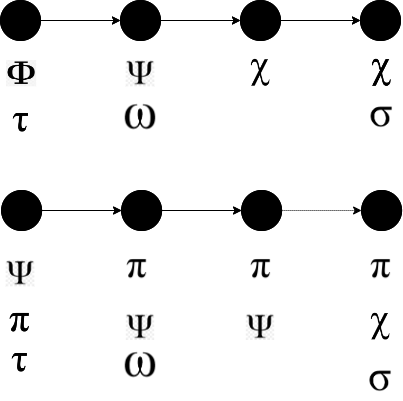
\includegraphics[width=0.9\textwidth, height = 10cm, keepaspectratio]{images/SOEN331_A4_Q6c.png}
\end{figure}
\\
\noindent Here we can see now that i+4 is removed and i + 3 is where the strong release ends and it \textbf{hence satisfies the behaviour for all requirements now}. \\

\item[(d)] (5 pts) Having resolved any possible conflicts in requirements, specify conditions
(models of behavior), if any exist, under which the program can terminate. If
none exist, please indicate so. \\
\\
\\
\\
\noindent \underline{Solution}:\\
There are two conditions in which the program terminates in: \\
\begin{enumerate}
\item[(1).]$\langle $ (\phi \wedge \tau),(\psi \wedge \omega), \chi, (\chi \wedge \sigma) $
\rangle$ \\
\item[(2).] $\langle $ (\psi \wedge \pi \wedge \tau), (\pi \wedge \psi \wedge \omega), (\pi \wedge \psi), (\pi \wedge \chi \wedge \sigma) $ \rangle$
\\
\end{enumerate}
\end{itemize}


\end{enumerate}





\end{spacing}

\end{document}